\documentclass{llncs}
\pagestyle{plain}
\usepackage{amsmath,amssymb,amsfonts,stmaryrd}
\usepackage{graphicx}
\usepackage[usenames,dvipsnames]{color}
\usepackage{tikz}
\usepackage{hyperref}
\usepackage[T1]{fontenc}
\usepackage{listings}
\usepackage{booktabs}
\usepackage{subfig}
\lstset{%
   basicstyle=\ttfamily, %\scriptsize\ttfamily,
%   frame=single,
   breaklines=true,
}
%\usepackage{algorithm}
\usepackage{float}

\newcommand{\wip}[1]{\textcolor{Purple}{WIPWIPWIPWIP #1 WIPWIPWIPWIP}}

\newif\ifcomments%

\commentstrue%
%\commentsfalse

\newcommand{\francois}[1]{\ifcomments\textcolor{blue}{#1}\fi}
\newcommand{\sylvain}[1]{\ifcomments\textcolor{green}{#1}\fi}
\newcommand{\arthur}[1]{\ifcomments\textcolor{brown}{#1}\fi}


\newcommand{\defleq}{\sqsubseteq_{\text{def}}}
\newcommand{\lra}{\longrightarrow}

\floatstyle{boxed}
\newfloat{listfig}{htb}{lstfig}
\floatname{listfig}{Listing}

\floatstyle{ruled}
\newfloat{algorithm}{htpb}{algfig}
\floatname{algorithm}{Algorithm}




\begin{document}

\title{Probably Approximately Correct Learning of Regulatory Networks from Time-Series Data}

\author{Arthur Carcano\inst{1} \and Fran\c{c}ois Fages\inst{2} \and Sylvain
Soliman\inst{2}}

\institute{%
Ecole Normale Sup\'erieure, Paris, France\\
  \email{arthur.carcano@ens.fr}
\and Inria, University Paris-Saclay, Lifeware group, France\\
   \email{Francois.Fages@inria.fr},
   \email{Sylvain.Soliman@inria.fr}
}

\maketitle

\begin{abstract}
Automating the process of model building from experimental data 
is a very desirable goal to palliate the lack of modellers for many applications.
However, despite the spectacular progress of machine learning techniques in data analytics, classification, clustering and prediction making,
learning dynamical models from data time-series is still challenging.
In this paper we investigate the use of the Probably Approximately Correct (PAC) learning 
framework of Leslie Valiant as a method for the automated discovery of influence models of biochemical processes from Boolean and stochastic traces. 
We show that Thomas' Boolean influence systems can be naturally represented by k-CNF formulae
and learned
from time-series data with a quasi linear number of Boolean activation samples per species,
and that positive Boolean influence systems can be represented by monotone DNF formulae
and learned actively with both activation samples and oracle calls.
We evaluate the performance of this approach on a model of T-lymphocyte
differentiation, with and without prior knowledge,
and discuss its merits as well as its limitations with respect to realistic experiments.
\end{abstract}

\section{Introduction}

Modelling biological systems is still an art which is currently limited in its applications by the number of available modellers.
Automating the process of model building is thus a very desirable goal
to attack new applications, develop patient-tailored therapeutics,
and also design experiments that can now be largely automated
with a gain in both the quantification and the reliability of the observations, at both the single cell and population levels.

Machine learning is revolutionising the statistical methods in biological data analytics,
data classification and clustering, and prediction making.
However, learning dynamical models from data time-series is still challenging.
A recent survey on probabilistic programming~\cite{GHNR14fose}
highlighted the difficulties associated with modelling time,
and concluded that existing frameworks are not sufficient in their treatment of dynamical systems.
There has been early work on the use of machine learning techniques, such as inductive
 logic programming~\cite{Muggleton95ngc} combined with active learning in the vision of the ``robot scientist''~\cite{BMOKRK01etai},
to infer gene functions,
metabolic pathway descriptions~\cite{AM02etai,AM02slps}
or gene influence systems~\cite{BCRG04jtb},
or to revise a reaction model with respect to CTL properties~\cite{CCFS06tcsb}.
Since a few years, progress in this field is measured on public benchmarks
of the ``Dream Challenge'' competition~\cite{Meyer14bmc}.
Logic Programming, and especially \emph{Answer Set Programming} (ASP), provide efficient tools such as CLASP~\cite{GKNS07lpnmr}
to implement learning algorithms for Boolean models.
They have been applied in~\cite{GSTUV08iclp} to the detection of  inconsistencies in large biological networks,
and have been subsequentially applied to the inference of gene networks from gene expression data and to the design of discriminant experiments~\cite{VKASSSG15frontiers}.
Furthermore, ASP has been combined with CTL model-checking in~\cite{OPSSG16biosystems} to learn mammalian signalling networks from time series data,
and identify erroneous time-points in the data.

Active learning extends machine learning with the possibility to call oracles, e.g.~make experiments,
and budgeted learning adds costs to the calls to the oracle.
The original motivation for the budgeted learning protocol came from medical applications in which the outcome of a treatment,
drug trial, or control group is known, and the results of running medical tests are each available for a price~\cite{DZBSM13ml}.
In this context, multi-armed bandit methods~\cite{DBSSZ07icdm} currently provide the best strategies.
In~\cite{LMALS14ecml}, a bandit-based active learning algorithm is proposed for experiment design in dynamical system identification.

In this paper, we consider the framework of Probably Approximately Correct (PAC) Learning 
which was introduced by Leslie Valiant in his seminal paper on a theory of the learnable~\cite{Valiant84cacm}.
Valiant questioned what can be learned from a computational viewpoint,
and introduced the concept of PAC learning,
together with a general-purpose polynomial-time learning protocol.
Beyond the algorithms that one can derive with this methodology,
Valiant's theory of the learnable has profound implications
on the nature of biological and cognitive processes,
of collective and individual behaviors,
and on the study of their evolution~\cite{Valiant13book}.

Here we present PAC learning as a possible basis to develop a method for the automated discovery of influence models of biochemical processes from time-series data. 
To the best of our knowledge, 
the application of PAC learning to dynamical models of biochemical systems has not been reported before.
We show that Thomas' gene regulatory networks~\cite{Thomas91jtb,Thomas73jtb} can be naturally represented by 
Boolean formulae in conjunctive normal forms with a bounded number of litterals (i.e.~k-CNF formulae),
and can be learned from Boolean transitions with a quasi linear number of Boolean transition samples, using Valiant's PAC learning algorithm for k-CNF formulae.
We also show that Boolean influence systems with their positive Boolean semantics discussed in~\cite{FMRS16cmsb}
can be naturally represented by monotone DNF formulae,
and learned actively from a set of positive samples with calls to an oracle.

In the following, these results\footnote{For the sake of reproducibility, the code used in this article is available at \url{http://lifeware.inria.fr/wiki/software/\#CMSB17}.} are first illustrated with a toy example, the Lotka-Volterra prey-predator system as running example,
and then on a Boolean influence model of 
the differentiation of the T-helper lymphocytes from~\cite{RRMTC06tcsb,Mendoza06biosystems},
composed of 32 influences and 12 variables.


\section{Preliminaries on PAC Learning}\label{pac}

\subsection{PAC Learning Protocol}

Let $n$ be the dimension of the model to learn, and let us consider a finite set of Boolean variables $x_1,\ldots,x_n$,
 A vector is an assignment of the $n$ variables to  $\mathbb{B} = \{0,1\}$;
 A Boolean function $G:{\mathbb{B}}^n \rightarrow \mathbb{B}$;
	assigns a Boolean value to each vector;


The idea behind the PAC learning protocol is to discover a Boolean function, $G$, which approximates a hidden function $F$, while restricting oneself to the two following operations~:
\begin{itemize}
  \item
\textsc{Sample}$()$: returns a positive example, i.e.~a vector $v$ such that $F(v)=1$.
The output of \textsc{Sample}$()$ is assumed to follow a given probability distribution $D(v)$, which is used to measure the approximation of the result.
  \item
\textsc{Oracle}$(v)$: returns the value of $F(v)$ for any input vector $v$.
\end{itemize}


\begin{definition}[\cite{Valiant84cacm}]\label{def:learnclass}
   A class $\cal M$ of \emph{Boolean functions} is said to be \emph{learnable}
   if there exists an algorithm $\cal A$ with some precision parameter $h\in\mathbb N$ such that:
   \begin{itemize}
      \item $\cal A$ runs in polynomial time both in $n$ and $h$;
      \item
         for any function $F$ in $\cal M$, and any distribution $D$ on the positive examples,
         $\cal A$ deduces with probability higher than $1-h^{-1}$ an approximation $G$ of $F$ such that
         \begin{itemize}
            \item $G(v)=1$ implies $F(v)=1$ (no false positive)
            \item
               $\displaystyle\sum_{v\ s.t.\ F(v)=1\wedge G(v)=0} D(v) < h^{-1}$ (low probability of false negatives)
         \end{itemize}
   \end{itemize}
\end{definition}

For the sake of simplicity, the same precision parameter $h$ is used above for quantifying both the \emph{probability} that the result is correct,
and the \emph{approximation} error tolerated in the correctness criterion.
We also limited ourselves to the case where vectors had all of their entries defined, but Valiant's work actually allows for only partially defined ones.


\subsection{PAC Learning Algorithms}

Valiant showed the learnability of some important classes of functions in this framework,
in particular for Boolean formulae in conjunctive normal forms with at most $k$ literals per conjunct (k-CNF),
and for monotone (i.e.~negation free) Boolean formulae in disjunctive normal form (DNF).

The computational complexity of the PAC learning algorithms for these classes of functions is expressed in terms of the function
$L(h,S)$ defined as the smallest integer $i$ such that
in $i$ independent Bernoulli trials, each with probability at least $h^{-1}$ of success, the probability of having fewer than $S$ successes is less than $h^{-1}$.
Interestingly, this function is quasi-linear in $h$ and $S$, i.e.~for all
integers $S\ge 1$ and reals $h>1$, we have $L(h,S) \le 2h(S+\log_e h)$~\cite{Valiant84cacm}.

\begin{theorem}[\cite{Valiant84cacm}]\label{thm:kcnf}
For any $k$, the class of $k$-CNF formulae on $n$ variables is learnable with an
algorithm that uses $L(h,{(2 n)}^{k+1})$ positive examples and no call to the
oracle.
\end{theorem}

The proof is constructive and relies on Alg.~\ref{algCNF} below. In this algorithm, the initialization of the learned function $g$ to the false constraint expressed as the conjunction of all possible \emph{clauses} (i.e.~disjunctions of litterals)
leads to the learning of a minimal generalization of the positive examples with mainly no false positive and low probability of false negatives.

\begin{algorithm}
\begin{enumerate}
  \item initialise $g$ to the conjunction of all the $(2n)^k$ possible clauses of at most $k$ literals,
\item do $L(h,(2n)^{k+1})$ times 
\begin{enumerate}
\item $v:=\textsc{Sample}()$
\item delete all the clauses in $g$ that do not contain a literal true in $v$
\end{enumerate}
\item output: $g$
\end{enumerate}
\caption{PAC-learning of $k$-CNF formulae.\label{algCNF}}
\end{algorithm}

In our implementation of the PAC-learning algorithm for $k$-CNF formulae,
we shall make use of the lattice structure of $k$-clauses ordered by implication.
Interestingly, this data structure allows for
\begin{itemize}
	\item $O(1)$ access to any $k$-clause;
	\item and for a clause $c$, $O(1)$ access to the smallest clauses implied by $c$ and to the biggest clauses that imply $c$.
\end{itemize}

The class of monotone DNF formulae is also learnable. Let the \emph{degree} of
a Boolean formula be the largest number of prime implicants (i.e., minimal
formulae covering one of the product-terms of the Boolean formula expressed as
a sum of products) in an equivalent rewriting of the formula as a
non-redundant sum of prime-implicants.


\begin{theorem}[\cite{Valiant84cacm}]\label{thm:mdnf}
    The class of monotone DNF formulae on $n$ variables is also learnable with an
    algorithm that uses $L(h,d)$ examples and $d n$ calls to the oracle,
    where $d$ is the \emph{degree} of the function to learn.
\end{theorem}

The proof relies on Alg.~\ref{algDNF}. As previously, the algorithm guarantees that a minimal generalization is learned from both the samples and the oracle.
The polynomial computational complexity follows from the fact that each monomial $m$ is a prime implicant
of $f$ by construction, and that it is constructed by at most $n$ calls to the
oracle.

\begin{algorithm}
\begin{enumerate}
\item initialise $g$ with false (constant zero),
\item
do $L(h,d)$ times 
\begin{enumerate}
\item $v:=\textsc{Sample}()$
	\item 
	if $v\Rightarrow g$ exit
\item for $i:=\ 1\ to \ n$
\begin{enumerate}
\item if $x_i$ is determined in $v$
\begin{enumerate}
\item $v^*:=v[x_i\leftarrow *]$
\item if $\textsc{Oracle}(v^*)$ then 
\begin{itemize}
\item $v:=v^*$
\item $m:=\bigwedge_{v\Rightarrow x_j} x_j\wedge\bigwedge_{v\Rightarrow\neg x_k}\neg x_k$ 
\item $g:=g\vee m$
\end{itemize}
\end{enumerate}
\end{enumerate}
\end{enumerate}
\item output: $g$
\end{enumerate}
\caption{PAC-learning of monotone DNF formulae.\label{algDNF}}
\end{algorithm}





\section{Influence Models of Molecular Cell Processes}

In this section, we present the formalism of influence systems used to model regulatory networks in cell molecular biology.
%and to which we will later whether or not PAC learning is applicable.
We assume again a finite set of molecular species $\{x_1,\dots,x_n\}$ 
and consider Boolean states that represent the activation or presence of each molecular species of the system, 
i.e.~vectors in $\mathbb{B}^n$ that specify whether or not the $i$th species is present, or the $i$th gene activated.

\subsection{Influence Systems with Forces}


Influence systems with forces have been introduced in~\cite{FMRS16cmsb}
to generalize the widely used logical models of regulatory networks \emph{\`a la} Thomas~\cite{Thomas73jtb},
in order to provide them with a hierarchy of semantics
including quantitative differential and stochastic semantics, similarly to reaction systems~\cite{FS08tcs}.

\begin{definition}[\cite{FMRS16cmsb}]
An \emph{influence system}
   $I$ is a set of quintuples $(P, I, t, \sigma, f)$ called \emph{influences}, noted in the examples below in Biocham v4\footnote{\url{http://lifeware.inria.fr/biocham4}} syntax,\\ \verb|f for P/I -> t| if $\sigma=+$, and \verb|f for P/I -< t| if $\sigma=-$,
   where 
\begin{itemize}
\item $P$ is a multiset on $S$, called \emph{positive sources} of the influence, 
\item $I$ a multiset of \emph{negative sources}, 
\item $t\in S$ is the \emph{target},
\item $\sigma\in\{+,-\}$ is the \emph{sign} of the influence, accordingly called either \emph{positive or negative influence},
\item and $f:\mathbb{R_+}^n\to\mathbb{R_+}$ is a function\footnote{More precisely, in a well-formed influence system, $f$ is assumed to be partially differentiable;
$x_i\in P$ if and only if $\sigma = +$ (resp.\ $-$) and
   ${\partial {f}}/ {\partial x_i}(\vec x)>0$ (resp.\ $<0$) for some value
   $\vec x\in\mathbb{R}_+^n$;
 and $x_i\in I$ if and only if $\sigma = +$ (resp.\ $-$) and
   ${\partial {f}}/ {\partial x_i}(\vec x)<0$ (resp.\ $>0$) for some value
  $\vec x\in\mathbb{R}_+^n$.}
called the \emph{force} of the influence.
\end{itemize}
\end{definition}

%In the examples below, the ASCII syntax of Biocham v4 is used for influences.
%Positive (resp.~negative) influences are written with an arrow \lstinline|->| (resp.~\lstinline+-<+)
%which separates the sources from the target.
%the positive and negative sources are separated
%by a \lstinline|/|, which can be omitted if there is no negative source.
The positive sources are distinguished from the negative sources of an influence (positive or negative),
in order to annotate the fact that in the differential semantics,
the source increases or decreases the force of the influence,
and in the Boolean semantics with negation whether the source, or the negation of the source,
is a condition for a change in the target.


\begin{example}\label{ex:LVi}
   The classical birth-death model of Lotka--Volterra can be represented by the following
influence system between a proliferating prey $A$ and a predator $B$:
  \lstinputlisting[firstline=6,lastline=9]{examples/LVif.bc}

\vspace{-2cm}\hfill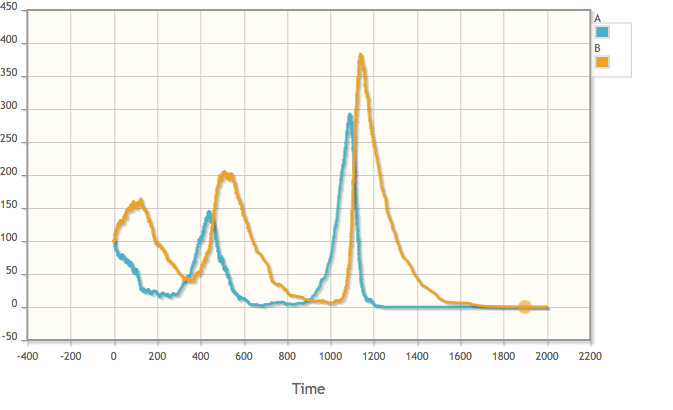
\includegraphics[width=0.45\textwidth]{LVstoch.png}

The influence forces can be used for differential or stochastic simulation as above.
This example contains both positive and negative influences but no influence inhibitor, i.e.~no negative source in the influences:
$(\{A, B\}, \emptyset, A, -, k1*A*B)$, $(\{A, B\}, \emptyset, B, +, k1*A*B)$, $(\{A\}, \emptyset, A, +, k2*A)$ and $(\{B\}, \emptyset, B, -, k3*B)$.
For an example of influence with inhibitor, one can consider the specific inhibition of the proliferation rate of $A$ by some variable $C$
(which is distinguished from a general negative influence of $C$ on $A$) by writing $C$ as an inhibitor of the positive influence of $A$ on $A$:
\verb|k2*A/(1+C) for A/C -> A.|
\end{example}



\begin{definition}[Boolean Semantics]
   The Boolean semantics (resp.~positive Boolean semantics) of an influence system $\{(P_i, I_i, t_i, \sigma_i,
   f_i)\}_{1\leq i\leq n}$
   over a set $S$ of $n$ variables,
   is the Boolean transition system $\lra$ defined over Boolean state vectors in $\mathbb{B}^n$
   by
   ${\vec x}\lra{\vec x'}$ if there exists an influence $(P_i, I_i, t_i, \sigma_i, f_i)$
   such that ${\vec x}\models \bigwedge_{p\in P_i} p\bigwedge_{n\in I_i} \neg n$ (resp.~${\vec x}\models \bigwedge_{p\in P_i} p$)
   and ${\vec x'} = {\vec x}\ \sigma_i\ t_i$.
\end{definition}


Equivalently, the Boolean semantics of an influence system over $n$ species, $x_1,\ldots,x_n$,
can be represented by $n$ activation and $n$ deactivation Boolean functions, 
 which determine the possible transitions from each Boolean state:

\begin{definition}[Boolean Activation Functions]\label{def:activation}
The \emph{Boolean activation functions} ${x_k}^+,\ {x_k}^-:{\{0,1\}}^n \rightarrow\{0,1\}$, $1 \leq k \leq n$,
of an influence system $\cal M$ are
$${x_k}^+=\bigvee_{(P,I,x_k,+,f)\in\cal M} \bigwedge_{p\in P_i} p\bigwedge_{n\in I_i} \neg n$$
$${x_k}^-=\bigvee_{(P,I,x_k,-,f)\in\cal M} \bigwedge_{p\in P_i} p\bigwedge_{n\in I_i} \neg n$$
The \emph{positive activation functions} are defined without negation by ignoring the inhibitors.
\end{definition}

Conversely any Boolean activation functions can be represented by an influence system
by putting the activation functions in DNF, and associating an influence to each conjunct.

Note that the positive Boolean semantics simply ignores the negative sources of an influence.
This is motivated by the abstraction and approximation relationships that link the Boolean semantics
to the stochastic semantics and to the differential semantics, for which the presence of an inhibitor decreases the force of an influence but does not prevent it to apply~\cite{FMRS16cmsb}.


\begin{definition}[Stochastic Semantics]\label{def:stoch}
   The stochastic semantics (resp.~positive stochastic semantics) of an influence system $\{(P_i, I_i, t_i,
   \sigma_i, f_i)\}_{1\leq i\leq n}$ over a set $S$ of $n$ variables, relies
   on the transition system $\lra$ defined over discrete states, i.e.\
   vectors in $\mathbb{N}^n$, by $\forall (P_i, I_i, t_i, \sigma_i, f_i), {\vec
   x}\lra{\vec x'} \text{ with propensity }f_i\text{ if }{\vec x}\geq P_i,
   {\vec x}<I_i$ (resp.~no condition on $I_i$) and ${\vec x'} = {\vec x}\  \sigma_i\ t_i$.
   Transition probabilities between discrete states are obtained through
   normalization of the propensities of all enabled transitions, and the time
   of next transition is given by an exponential distribution~\cite{Gillespie77jpc}.
\end{definition}

We call a positive influence system, an influence system without inhibitors or interpreted under the positive semantics.

\subsection{Monotone DNF Representation of Positive Influence Systems}

Def.~\ref{def:activation} shows how to represent an influence system by $2*n$ activation functions in DNF, 
and positive influence systems by monotone DNF activation functions.

\begin{example}
The activation functions of the Lotka--Volterra influence system of Ex.~\ref{ex:LVi}
are monotonic DNF formulae with only one conjunct since in this example there is only one signed influence per variable:
\begin{align*}
   A^+&=(A)& B^+&=(A\wedge B)\\
   A^-&=(A \wedge B)& B^-&=(B)
\end{align*}

\end{example}

%Note that in Ex.~\ref{ex:lympho} no (de)activation function is monotone.

\subsection{$k$-CNF Representation of General Influence Systems}
\label{sec:kcnf}

Monotone DNF formulae cannot encode the Boolean dynamics of influence systems with negation,
which tests the absence of inhibitors, i.e. their negation.
This is possible using a $k$-CNF representation of the activation functions,
provided that there are at most $k$ species that can play a given ``role''. 
For instance, in a hypothetic activation function in CNF
$
\left(a \vee b \vee c\right) \bigwedge
\left(d \vee e\right) \bigwedge 
\neg f
$,
each clause can be interpreted as a role, and each role can be played by a limited number of species, at most $k$.
%for the activation of our hypothetic gene, we need at least one species that plays this role. For example, the enzyme can be $a$, $b$, or $c$ whereas 
%the reactant is $d$ or $e$, and we need that $f$ be inactive.


\begin{example}
   The activation functions of the prey-predator model with inhibition of Ex.~\ref{ex:LVi} cannot be
   represented by monotone formulae. They can however be represented by the following 1-CNF
   formulae ($k=1$ since there is only one positive and one
   negative influence for each target):
\begin{align*}
   A^+&=(A)\wedge(\neg C)& A^-&=(A) \wedge (B)\\
   B^+&=(A)\wedge (B)& B^-&=(B)
\end{align*}

\end{example}

\begin{example}
   In Sec.~\ref{ex:lympho}, we shall study a model of T lymphocyte differentiation which contains 2-CNF activation functions, for instance
   \[\text{IFNg}^+=(\text{STAT4}\vee \text{TBet})\qquad
   \text{IFNg}^-=(\neg \text{STAT4})\wedge(\neg \text{TBet})\]
\end{example}

\subsection{$k$-CNF Models of Thomas Functional Influence Systems}


\begin{definition}[\cite{Thomas73jtb}]
   A \emph{Thomas} network on a finite set of genes $\{x_1,\dots,x_n\}$
   is defined by  $n$ Boolean functions $\{f_1,\dots,f_n\}$ which give for each gene its
   possible next state, given the current state.
\end{definition}

The difference with the previous general influence systems
is that the activation and deactivation functions are exclusive and defined by one single function.
%As proven in~\cite{FMRS16cmsb}, in the Boolean setting any influence system is
%also a Thomas' network.
%FF non on montre justement le contraire !
%As this will be useful later on, we also remark that the Thomas' Network can
%be computed from the (de)activation functions presented in Def.~\ref{def:activation} by:
As shown in~\cite{FMRS16cmsb}, non-terminal self-loops cannot be represented in Thomas functional influence systems.
Given a general influence system with activation functions ${x_i}^+$ and ${x_i}^-$, one can associate a Thomas network 
with attractor function\footnote{Note that this function ignores the cases where $v_i = 0$ and ${x_i}^-(v) =0$, or $v_i=1$ and ${x_i}^+(v)=1$
which may create loops in non-terminal states in general influence systems.}
\[
f_i(v) = \left\{\begin{array}{l}
1 \text{ if } \left\{\begin{array}{l}
v_i = 0 \text{ and } {x_i}^+(v) = 1\\
v_i = 1 \text{ and } {x_i}^-(v) = 0 \\
\end{array}\right.\\[1em]
0 \text{ if } \left\{\begin{array}{l}
v_i = 0 \text{ and } {x_i}^+(v) = 0\\
v_i = 1 \text{ and } {x_i}^-(v) = 1\\
\end{array}\right.
\end{array}\right.
\]

$k$-CNF formulae can again be used to represent Thomas gene regulatory network functions with some reasonable restrictions on their connectivity.
In particular, it is worth noticing that in Thomas networks of degree bounded by $k$,
each gene has at most $k$ regulators, each gene activation function $f_i$ thus depends of at most $k$ variables
and can consequently be represented by a $k$-CNF formula.

\begin{example}
   The above translation applied to
   Ex.~\ref{ex:LVi} gives
   \[f_A = A \wedge\neg B\qquad f_B = 0\]
   Note that the form of $f_B$ means that the only possible state change
   for $B$ is from $1$ to $0$. 
%Of course $B$ can also stay at $1$ but
%non-terminal self-loops are not representable in Thomas logical models \cite{FMRS16cmsb}.
\end{example}

\begin{example}
   The T-lymphocyte model studied in Sec.~\ref{ex:lympho} is originally a Thomas' network, where we have, for
   instance:
   \[f_\text{IFNg}=(\text{STAT4}\vee \text{TBet})\]
\end{example}

\section{PAC Learning from Traces} %Experimental Setup}

%To further discuss the applicability of PAC learning to actual experiments, we hereby introduce what we believe is a plausible experimental setup, and discuss its implications on the learning of different classes of functions.

\subsection{Steps and Traces}

In practice, one cannot assume to have full access to the hidden Boolean function as required by
\textsc{Sample} and \textsc{Oracle}, but rather to data time-series, or traces,
produced from biological experiments. At this point of the discussion we would like to remind our reader that our goal is not to assess the usability of PAC learning as is to learn models from real data traces, but rather to show that it is of interest to our community, and give some leads on how it should be approached by people willing to study it deeper.

More specifically, and as illustrated in Fig.~\ref{steps}, we consider that the experimental setup we are going to simulate enables us to identify a ``step'' of its evolution, i.e.~that we are able to obtain a trace $(v_i)_{0 \leq t \leq T}$ of the Boolean state of activation of its species where for all $t$ in $[0,T-1]$, $v_t$ and $v_{t+1}$ differ in exactly one coordinate. That is, the state of exactly one species has changed.
Even though we will finally not require it, we first also consider that our experimental setup enables us to put the system in a given state, i.e.~that for any $v \in \mathbb{B}^n$ we can set the experiment's initial conditions so that they are correctly abstracted by $v$.


\begin{figure}[htbp]
	{\large 
	\[
	\cdots
	\rightarrow
	\underset{\vspace{1em}(a)}{
		\left(\begin{array}{c}
		0\\ 1\\ 0\\ 1
		\end{array}\right)}
	\rightarrow
	\underset{\vspace{1em}(b)}{
		\left(\begin{array}{c}
		\textbf{\textit{1}}\\ 1\\ 0\\ 1
		\end{array}\right)}
	\rightarrow
	\underset{\vspace{1em}(c)}{
		\left(\begin{array}{c}
		1\\ 1\\ 0\\ \textbf{\textit 0}
		\end{array}\right)}
	\rightarrow
	\cdots
	\]
}
	\caption{\label{steps}Illustration of a hypothetical experimental setup with three steps of a trace. Between $a$ and $b$, the first gene has been activated, and between $b$ and $c$, the last one has been deactivated.}
\end{figure}



\subsection{Sample and Oracle on  Traces}
%Now that our hypothetical experimental setup is described, we will discuss how the two key operations of PAC-learning (\textsc{Sample} and \textsc{Oracle}) can be implemented, if at all, in it.

%Because both influence systems and \textit{\`{a} la Thomas} networks essentially boil down to activation and deactivation functions we limit ourself to those in the following.

\subsubsection{Sampling.}

It is worth remarking that sampling of activation and deactivation functions is easy in this setting. Referring to Fig.~\ref{steps}, $(a)$ is a positive example for the activation function ${x_1}^+$, and $(b)$ for ${x_4}^-$.
A call to \textsc{Sample} can then simply be a search in the trace for the next positive example for the current function, shall it exist.
PAC learning will associate a guarantee on the quality of each learnt Boolean
function ($h$) depending on the number of samples used $L(h, (2n)^{k+1})$,
where $n$ is the number of genes/molecules observed, and $k$ is a parameter of
the learning procedure as explained in Section~\ref{sec:kcnf}.
In practice, $k$ can be limited to 3 (2 was the max we observed) and $2n$, the
number of different possible literals in a clause, can also be reduced through
prior knowledge (see Section~\ref{sec:prior}).

The global guarantee on the learnt model is the minimum of all observed $h$,
it is therefore crucial to have as diverse samples as possible. This can be
achieved by running several traces from different initial states,
as discussed in more details in an example in Section~\ref{sec:abinitio}.

\subsubsection{Oracle.}
The \textsc{Oracle} function needs to evaluate the (de)activation function on a given vector $v$, that is, it needs to be able to set the system in a state abstracted by $v$ and say whether or not a given gene can be (de)activated from this state.
The intuitive solution is the following: set the system in the desired state and see whether or not the gene is (de)activated. 
However, different atomic steps are possible from a given state and we have no guarantee that the one we are interested in will happen if we run this scheme once. The only way to have such a guarantee would be to perform this an infinite number of time.
Since actually running this ``set the state and observe the first atomic step'' scheme an infinite number of time is impossible, extending the historical PAC-learning framework with ways to use an oracle that is only probabilistic arise as one of the first improvements that should be worked on.
%A peculiarly fast-thinking reader may also have notice that different (and often infinitely many) states of the system may also be abstracted by the same Boolean total vector $v$, and that the transition may also happen from only some of them.
%For those reasons, algorithm requiring the \textsc{Oracle} function seem not applicable as of today, and we choose to only focus on $k$-CNF and sampling from now on.


%\section{In sillico application}
\subsection{PAC Learning from Boolean Traces}

A first experiment was to simulate Boolean traces for a given influence network, and use them as a basis to learn.
We report results on our running
Ex.~\ref{ex:LVi}., but to increase readability we used long names for the
species (populations) as shown in Listing~\ref{bool-LV}.
The results are presented in Fig.~\ref{bool-LV.res}.

%\subsubsection{Results}
\begin{listfig}[htp]
	\lstinputlisting{examples/LVi.bc}
   \caption{The Lokta-Voltera prey vs.\ predator model of Ex.~\ref{ex:LVi}
   with explicit names.\label{bool-LV}}
\end{listfig}%
\begin{figure}[htp]
   \begin{minipage}{.5\textwidth}
      \lstinputlisting{examples/bool-lokta.res}
   \end{minipage}%
   \vrule\hspace{.04\textwidth}
   \begin{minipage}{.45\textwidth}
      \begin{lstlisting}
Predator / Prey -< Predator
Predator, Prey -< Prey
      \end{lstlisting}
   \end{minipage}
   \caption{Results of PAC-learning on a single trace of length 50 of the Boolean simulation of the
   Lokta--Voltera example. Left pane shows the actual Boolean functions
learnt (where \texttt{!A} stands for $\neg A$), and right pane the corresponding influence system.}\label{bool-LV.res}
\end{figure}

The inferred model can be interpreted as follows.
%
Both the predator and the prey species cannot appear. It is important to note that the activation functions in the Lokta--Voltera models reports the apparition on extinction of the species' population as a whole and not of individuals of it.
%
For the predator to disappear, it is necessary that there is a predator in the first place and that there is no prey. If the first part of this conjunction is obviously true, the second is false: strictly speaking, predators may disappear even if there are preys left, yet this case is very unlikely: the most likely case is that the predator will go extinct only once there are no more preys left for it to eat. This is a good example of how the learning is only approximate.
%
Finally, for the prey to go extinct, there must be both a prey in the first place and a predator to eat it. This is correct.


As can be seen even on this very simple example, the ``approximately'' in PAC has a precise meaning. Yet, as explained in Def.~\ref{def:learnclass}, the quantification of this approximation relies on the knowledge of the distributions of the samples.
%
In the present case, the probability of a positive example $v$ of (de)activation function $x\pm$ to be sampled is strongly and intuitively correlated to both the probability that the system reaches state $v$ and the probability of the actual (de)activation of gene $x$ from state $v$. 

Note that to obtain the output above, a single Boolean simulation was used.
Replacing it with 25 simulations of length 2 allows one to find the original
function for the inhibition of the predator (\texttt{Predator -< Predator}).
This role of the diversity of the initial states on the repartition of the
samples will be explored in more depth in the following sections.


\subsection{PAC Learning from Stochastic Traces}

Let us now consider stochastic traces
produced from the hidden model, using Gillespie's
algorithm for the simulation of the stochastic semantics given in
Def.~\ref{def:stoch}.

In general, we will assume mass-action kinetics with rate 1 for all reactions.
The initial states are random, but with equal probability to be 0 or $>0$ in
order to facilitate the observation of inhibited reactions.

The traces obtained are in ${\mathbb{N}}^n$, they are then abstracted to
Boolean samples by the usual $\{0, >0\}$ abstraction for the states, and the
increasing/decreasing abstraction for choosing samples for the
activation/deactivation functions. Using the same $\{0, >0\}$ abstraction to
detect samples would again forbid to learn autocatalytic influences like
\texttt{Prey -> Prey} for the same reason as in the Boolean case.

\begin{listfig}[htp]
   \begin{lstlisting}
biocham: pac_learning('library/examples/lotka_volterra/LVi.bc', 50, 1).
% Maxmimum K used: 1
% minimum number of samples for h=1: 18

% 14 samples (max h ~ 0.7777777777777778)
Predator -< Predator

% 7 samples (max h ~ 0.3888888888888889)
Predator,Prey -> Predator

% 1 samples (max h ~ 0.05555555555555555)
Predator,Prey -< Prey

% 21 samples (max h ~ 1.1666666666666667)
Prey -> Prey
   \end{lstlisting}
   \caption{Biocham running the PAC learning algorithm on the Lotka--Volterra
      model by generating 50 random initial states from which a stochastic
      simulation of length 1 is run to obtain samples. Among those 50 initial
     states, 7 had both prey and predator absent, leading to no sample.}%
   \label{lst:stoch_lv}
\end{listfig}

As shown by the run in Listing~\ref{lst:stoch_lv}, even with a low number of
samples (and therefore a very low $k$), one can find the full model with 50
simulations of length 1, all starting from random initial states.
A more detailed discussion of the role of the diversity of initial states is
given in Section~\ref{sec:abinitio}.

\section{Evaluation on a Model of T-helper Lymphocytes Differentiation}\label{ex:lympho}

%All the systems proposed so far were of humble size. 

In this section we evaluate the performance of the $k$-CNF PAC learning
algorithm on an influence system of 12 variables and 32 influences that models
the differentiation of the T-helper lymphocytes.
All learning experiments described below run on a
low-end laptop in less than 3s.

\subsection{Boolean Thomas Network}

This model, presented in~\cite{RRMTC06tcsb} is actually a Boolean
simplification of the original multi-level model
of~\cite{Mendoza06biosystems}. It studies the regulatory network of stimuli
leading to differentiation between Th-1 and Th-2 lymphocytes from an original
CD4+ T helper (Th-0).
The model has three different stable states corresponding to Th-0 (naive
lymphocyte), Th-1 and Th-2 when IL12 is off, and two others when IL12 is on
(the Th-0 one is lost).

\begin{figure}[htbp]
   \centering
   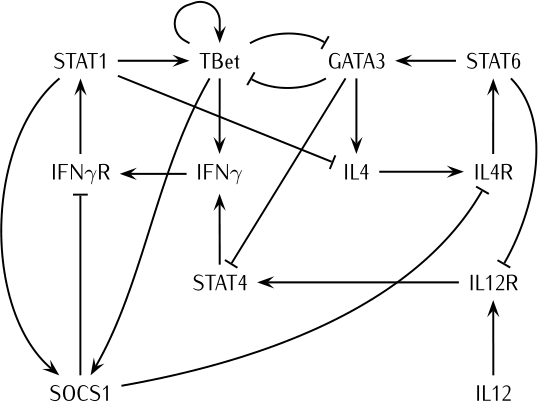
\includegraphics[width=0.8\textwidth]{th_net_clean.png}
   \caption{Fig.~4 of~\cite{RRMTC06tcsb} displaying the Th-lymphocyte
   differentiation model.\label{fig:lympho}}
\end{figure}

Fig.~\ref{fig:lympho} shows the influence graph of the model. The
corresponding code is given in appendix (Listing~\ref{bool-lympho}).

\subsection{\emph{Ab initio} PAC Learning from Boolean Traces}
\label{sec:abinitio}

Results of learning on the traces resulting from the Boolean simulation of this system from one single initial state gave results that were hardly readable for the human experimenter. Whether they were still good at predicting the behavior of the model is not obvious. On the one hand, guarantees on this come directly from Valiant's work with the approximation bounds, on the other hand,  
Valiant's results stand only if we actually have at least $L$ samples for each of the (de)activation functions, where $L$ is Valiant's bound. A first naive approach might be to simply let the trace run for $2nL$ steps, or a constant factor of it. Unfortunately, the repartition of samples for each function can be pretty non-uniform, as illustrated in Fig.~\ref{nsample-tab}. Hence, we would have to find a system to track the number of samples collected so far for each function, but without running infinitely long shall one gene be never (de)activated.

%Thankfully, the PAC learning algorithm for $k$-CNF can be modified to be able to take hints into account.

This entices us to find way to make the learning more precise. A first possibility is to aggregate samples resulting from multiple runs, done from random starting points. For example 140 runs provides a significant improvement, as the output is now more or less readable, as displayed in Listing~\ref{lympho-rand.res}. Note that randomizing does not really make the repartition of the samples more uniform, as shown in Fig.~\ref{nsample-tab2}. We can also remark that -- for the same number of steps -- there is not necessarily more \emph{different} samples when randomizing periodically the state (ie, restarting with random conditions) than when not doing it, as shown Fig.~\ref{eff-samp}. Yet, the quality of learning is better when doing periodic random reinitialization, leading us to believe that even if there is not more different samples, they are distributed in a way that cover more exhaustively the behavior of the system.

\sylvain{not sure if all this is not biased by the spurious added
activations/inhibitions. See Fig.~\ref{fig:statistics}.}

\subsection{PAC Learning with Prior Knowledge on the Influence Graph}
\label{sec:prior}

Even with such improved results, the obtained model remains approximate, and
it becomes obvious that with much bigger examples, the amount of data needed
to get back the initial model would become huge.
Machine learning with prior knowledge can save a lot of work by constraining the possible results and pruning the search.

Here we want the user to be able to specify, for each gene $x$, a set of gene $V_x$ which are the only ones on which $x^+$ and $x^-$ may depend. If one views the influences as a graph, this is akin to specifying a set of possible (undirected) edges outside of which the algorithm cannot build its influence system. Example of such hints for the lymphocyte model are given in Listing~\ref{hints}. 

It is remarkable than when given such prior knowledge, the model becomes fully readable for the experimenter, and provides them with information on the exact structure of the influences, as shown in Listing~\ref{hints.res}.




\section{Conclusion and Perspectives}

We have shown that Valiant's work on PAC learning provides an elegant trail 
to attack the challenge of inferring the structure of influence models from the observation of data time series,
and more precisely to automatically discover possible regulatory networks of a biochemical process, given sufficiently precise observations of its executions.

The Boolean dynamics of biochemical influence systems, including Thomas regulatory networks, can be represented by $k$-CNF formulae without loss of generality,
and $k$-CNF PAC learning algorithm can be used to infer the structure of the network from
a sufficiently large and diverse set of state transition traces.
When dimension increases, we have shown on an example of T-lymphocyte differentiation from the literature
that the $k$-CNF PAC learning algorithm can also leverage available
prior knowledge on the system to deliver precise results with a reasonable
amount of data.

The Boolean dynamics of positive influence systems can also be straightforwardly represented by monotone DNF activation and deactivation functions,
and monotone DNF PAC learning algorithm applied with an interesting recourse to oracles 
which are particularly relevant in the perspective of online active learning and experimental design.

More work is needed however to make comparisons on common benchmarks
with  other approaches already investigated in this context, such as Answer Set Programming (ASP) and budgeted learning,
and to investigate the applicability of these methods to real experiments taking into account particular biological technologies.

\bibliographystyle{splncs03}
\bibliography{contraintes}
\newpage
\section*{Appendix}
\begin{listfig}[H]
\lstinputlisting{examples/lympho-bool.reac}
\caption{Code for the lymphocyte differentiation of example~\ref{ex:lympho}.\label{bool-lympho}}
\end{listfig}


\begin{figure}[htbp]
	\centering
	\subfloat[Single trace.\label{nsample-tab}]{\hspace{1ex}%
	$$
	\begin{tabular}{l r}
	\toprule	     
	Function &  Number of samples\\
	\midrule
	GATA3-   &    360 \\
	GATA3+   &    361 \\
	STAT6-   &    546 \\
	STAT6+   &    547 \\
	STAT4+   &    805 \\
	STAT4-   &    805 \\
	IL12R-   &    849 \\
	IL12R+   &    849 \\
	IL4R-    &    862 \\
	IL4R+    &    863 \\
	IL12+    &   1096 \\
	IL12-    &   1096 \\
	IL4-     &   2204 \\
	IL4+     &   2205 \\
	TBet-    &   7135 \\
	TBet+    &   7135 \\
	STAT1+   &   9359 \\
	STAT1-   &   9359 \\
	IFNgR+   &  12026 \\
	IFNgR-   &  12026 \\
	SOCS1+   &  12600 \\
	SOCS1-   &  12600 \\
	IFNg-    &  25103 \\
	IFNg+    &  25103 \\
	\bottomrule
	\end{tabular}
	$$\hspace{1ex}
%	\caption{Repartition of samples in a simulation of the lymphocyte influence system for a single trace. Coefficient of variation is around 1.2.\label{nsample-tab}}	
}\hspace{5ex}
\subfloat[100 traces, random starting points.\label{nsample-tab2}]{\hspace{1ex}%
$$
\begin{tabular}{lr}
\toprule
Function &  Number of samples\\
\midrule
GATA3+   &    3861 \\
GATA3-   &    3869 \\
STAT6+   &    5614 \\
STAT6-   &    5621 \\
STAT4+   &    7980 \\
STAT4-   &    8010 \\
IL12R+   &    8420 \\
IL12R-   &    8446 \\
IL4R+    &    8665 \\
IL4R-    &    8671 \\
IL12-    &   10651 \\
IL12+    &   10651 \\
IL4-     &   21888 \\
IL4+     &   21889 \\
TBet+    &   69134 \\
TBet-    &   69164 \\
STAT1+   &   91070 \\
STAT1-   &   91114 \\
IFNgR+   &  116681 \\
IFNgR-   &  116721 \\
SOCS1+   &  122546 \\
SOCS1-   &  122589 \\
IFNg+    &  242331 \\
IFNg-    &  242357 \\
\bottomrule
\end{tabular}
	$$\hspace{1ex}
%	\caption{Repartition of samples in a simulation of the lymphocyte influence system for a hundred traces with random starting points. Coefficient of variation is still around 1.2.\label{nsample-tab2}}
}
\caption{Repartition of samples in a simulation of the lymphocyte influence system with varying number of traces. The coefficient of variation is around 1.2 in both cases. Rows are sorted by number of samples.}
\end{figure}

\begin{listfig}[htb]
	\lstinputlisting{examples/lympho_100_2_140.res}
	\caption{Results of PAC learning on 140 simulation of the lymphocyte influence system, with random starting points.\label{lympho-rand.res}}
\end{listfig}

\begin{figure}[htbp]
	\[
\begin{tabular}{lrr}
\toprule
Function &  No random restart &      Random restart \\
\midrule
IL12+    &   0.7 &   0.7 \\
IL12-    &   1.1 &   1.0 \\
IL4+     &   0.8 &   0.9 \\
IL4-     &   1.5 &   1.5 \\
STAT4+   &   0.6 &   0.7 \\
STAT4-   &   3.6 &   3.6 \\
IFNg+    &   0.1 &   0.1 \\
IFNg-    &   0.2 &   0.2 \\
TBet+    &   0.2 &   0.2 \\
TBet-    &   0.2 &   0.2 \\
GATA3+   &   3.2 &   3.3 \\
GATA3-   &   2.8 &   2.9 \\
STAT1+   &   0.2 &   0.2 \\
STAT1-   &   0.2 &   0.2 \\
IFNgR+   &   0.1 &   0.1 \\
IFNgR-   &   0.2 &   0.3 \\
SOCS1+   &   0.2 &   0.3 \\
SOCS1-   &   0.2 &   0.2 \\
IL4R+    &   1.0 &   1.1 \\
IL4R-    &   2.9 &   3.1 \\
IL12R+   &   1.3 &   1.2 \\
IL12R-   &   2.8 &   2.7 \\
STAT6+   &   1.9 &   2.1 \\
STAT6-   &   3.3 &   3.7 \\
\bottomrule
\end{tabular}
	\]
	\caption{Percentages of samples that have never been seen before, for each function.\label{eff-samp}}
\end{figure}

\begin{listfig}[htb]
	\lstinputlisting{examples/lympho.hints}
	\caption{Prior knowledge for the lymphocyte model. For each species, a set of possible influencers is given. The PAC algorithm will then learn a model in which only the specified influencers can either induce or inhibit the species.\label{hints}}
\end{listfig}



\begin{listfig}
	\lstinputlisting{examples/lympho-bool.res}
	\caption{Results for lymphocyte model, with prior knowledge on the unlabeled influence graph.\label{hints.res}}
\end{listfig}

\begin{figure}[htb]
   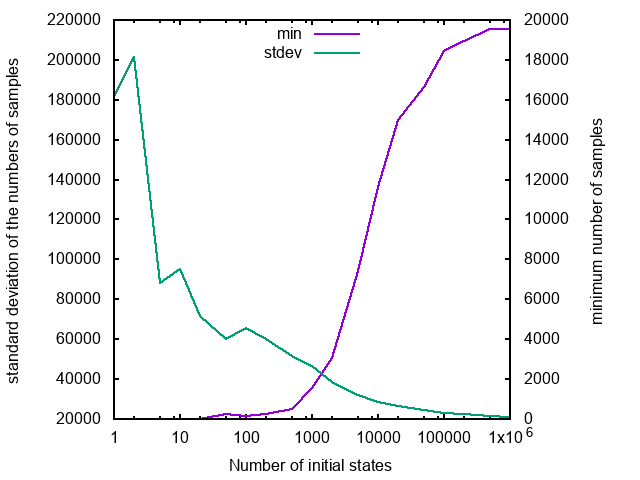
\includegraphics[width=\textwidth]{statistics/statistics.png}
   \caption{Evolution of the standard deviation and of the minimum number of
   samples for the 24 boolean functions of the Th-lymphocyte example. The
minimum gives a quasi-linear estimate of the confidence $h$. The total (and
therefore the average) number of samples is kept constant by adjusting the
time horizon of the simulations. Obviously, more diverse initial states (e.g.,
mutants) reveals more about the model structure than longer experiments.}%
\label{fig:statistics}
\end{figure}
\end{document}
